
%(BEGIN_QUESTION)
% Copyright 2014, Tony R. Kuphaldt, released under the Creative Commons Attribution License (v 1.0)
% This means you may do almost anything with this work of mine, so long as you give me proper credit

Complete the following table of values for this circuit, expressing each quantity in both rectangular and polar forms:

$$\includegraphics[width=15.5cm]{i03044x01.eps}$$

% No blank lines allowed between lines of an \halign structure!
% I use comments (%) instead, so that TeX doesn't choke.

$$\vbox{\offinterlineskip
\halign{\strut
\vrule \quad\hfil # \ \hfil & 
\vrule \quad\hfil # \ \hfil & 
\vrule \quad\hfil # \ \hfil & 
\vrule \quad\hfil # \ \hfil \vrule \cr
\noalign{\hrule}
%
% First row 
 -- -- & $L$ & $C$ & Total \cr
%
\noalign{\hrule}
%
% Another row
$V$ (polar) & \hskip 75pt & \hskip 75pt & 600 V $\angle$ 0$^{o}$ \cr
$V$ (rect.) &  &  & 600 + j0 V  \cr
%
\noalign{\hrule}
%
% Another row
$I$ (polar) &  &  & \hskip 75pt \cr
$I$ (rect.) &  &  &   \cr
%
\noalign{\hrule}
%
% Another row
$Z$ (polar) &  &  &   \cr
$Z$ (rect.) &  &  &   \cr
%
\noalign{\hrule}
} % End of \halign 
}$$ % End of \vbox


\underbar{file i03044}
%(END_QUESTION)





%(BEGIN_ANSWER)

\noindent
{\bf Partial answer:}

% No blank lines allowed between lines of an \halign structure!
% I use comments (%) instead, so that TeX doesn't choke.

$$\vbox{\offinterlineskip
\halign{\strut
\vrule \quad\hfil # \ \hfil & 
\vrule \quad\hfil # \ \hfil & 
\vrule \quad\hfil # \ \hfil & 
\vrule \quad\hfil # \ \hfil \vrule \cr
\noalign{\hrule}
%
% First row 
 -- -- & $L$ & $C$ & Total \cr
%
\noalign{\hrule}
%
% Another row
$V$ (polar) & 600 V $\angle$ 0$^{o}$ & 600 V $\angle$ 0$^{o}$ & 600 V $\angle$ 0$^{o}$ \cr
$V$ (rect.) & 600 + j0 V & 600 + j0 V & 600 + j0 V \cr
%
\noalign{\hrule}
%
% Another row
$I$ (polar) &  & 2.398 A $\angle$ 90$^{o}$ &  \cr
$I$ (rect.) & 0 $-$ j3.183 A &  & 0 $-$ j0.785 A \cr
%
\noalign{\hrule}
%
% Another row
$Z$ (polar) & 188.5 $\Omega$ $\angle$ $90^{o}$ &  & 763.9 $\Omega$ $\angle$ 90$^{o}$ \cr
$Z$ (rect.) &  & 0 $-$ j250.2 $\Omega$ &  \cr
%
\noalign{\hrule}
} % End of \halign 
}$$ % End of \vbox



%(END_ANSWER)





%(BEGIN_NOTES)

% No blank lines allowed between lines of an \halign structure!
% I use comments (%) instead, so that TeX doesn't choke.

$$\vbox{\offinterlineskip
\halign{\strut
\vrule \quad\hfil # \ \hfil & 
\vrule \quad\hfil # \ \hfil & 
\vrule \quad\hfil # \ \hfil & 
\vrule \quad\hfil # \ \hfil \vrule \cr
\noalign{\hrule}
%
% First row 
 -- -- & $L$ & $C$ & Total \cr
%
\noalign{\hrule}
%
% Another row
$V$ (polar) & 600 V $\angle$ 0$^{o}$ & 600 V $\angle$ 0$^{o}$ & 600 V $\angle$ 0$^{o}$ \cr
$V$ (rect.) & 600 + j0 V & 600 + j0 V & 600 + j0 V \cr
%
\noalign{\hrule}
%
% Another row
$I$ (polar) & 3.183 A $\angle$ $-90^o$ & 2.398 A $\angle$ 90$^{o}$ & 0.785 A $\angle$ $-90^o$ \cr
$I$ (rect.) & 0 $-$ j3.183 A & 0 + j2.398 A & 0 $-$ j0.785 A \cr
%
\noalign{\hrule}
%
% Another row
$Z$ (polar) & 188.5 $\Omega$ $\angle$ $90^{o}$ & 250.2 $\Omega$ $\angle$ $-90^o$ & 763.9 $\Omega$ $\angle$ 90$^{o}$ \cr
$Z$ (rect.) & 0 + j188.5 $\Omega$ & 0 $-$ j250.2 $\Omega$ & 0 + j763.9 $\Omega$  \cr
%
\noalign{\hrule}
} % End of \halign 
}$$ % End of \vbox

%INDEX% Electronics review: AC reactance and impedance
%INDEX% Electronics review, phasor expressions of circuit quantities
%INDEX% Electronics review: series and parallel AC circuits

%(END_NOTES)


